\section{Zielsetzung}
In diesem Versuch wird ein Germanium Energiedetektor mit einer geeichten
152Eu Quelle kalibriert. Der kalibrierte Detektor wird anschließend
verwendet um das Spektrum einer monochromatischen 137Cs Quelle aufzunehmen.
Danach wird mit dem Spektrum einer 133Ba Quelle deren Aktivität bestimmt.
Schließlich wird anhand eines weiteren Spektrums eine unbekannte Quelle 
identifiziert.


% Stichworte:
% \begin{itemize}
% \item Vollenergienachweiswahrscheinlichkeit
% \item Linien des Eu Spektrums
% \item Halbwertsbreite
% \item Compton Kante \item
% \end{itemize}

%---------------------------------------------------------------------------------------------------------------------------------------------------------------%

\section{Theorie}
\subsection[]{Wechselwirkung von Strahlung mit Materie}
Die Interaktionswahrscheinlichkeit von Gamma Strahlen mit Materie lässt sich
durch den Dämpfungskoeffizienten $\mu$ darstellen. Die Strahlungsintensität
fällt in dichten Materialien exponentiell ab $I ~ \exp(-\mu x)$. Dieser
Intensitätsverlust hängt direkt mit der Wirkungsquerschnitt des materials
zusammen und ist in $\mu$ eine additive Größe. Die Dämpfungskoeffizienten von
Gammastrahlen sind in Abbildung \ref{fig:mu} zu sehen. Abbildung \ref{fig:z}

\begin{figure}
	\centering
	\begin{subfigure}{.5\textwidth}
		\centering
		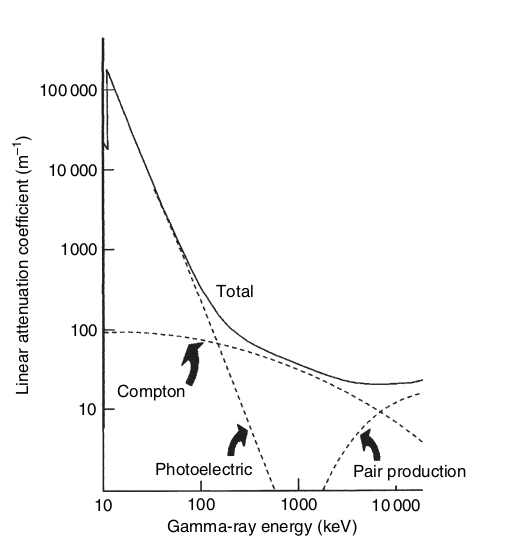
\includegraphics[width=0.9\linewidth]{./Bilder/E_mu_Gilmore.png}%
		\caption{Linearer Dämpfungskoeffizient aus \cite{book:gil}.}\label{fig:mu}
	\end{subfigure}%
	\begin{subfigure}{.5\textwidth}
		\centering
		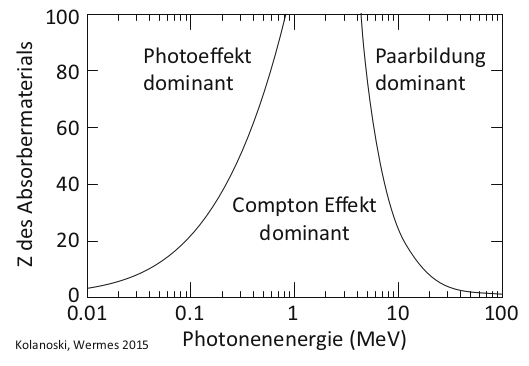
\includegraphics[width=0.9\linewidth]{./Bilder/E_Z_Kolanoski.png}
		\caption{Dominante Effekte nach $E_\gamma$ und $Z$ aus \cite{book:kolano}.}\label{fig:z}
	\end{subfigure}
	\caption{Interaktionswahrscheinlichkeiten von Gammastrahlen in verschiedenen Darstellungen.}\label{}
\end{figure}

Aus \cite{book:gil}. Die hauptsächlichen Wechselwirkungen von Photonen mit
Materie sind die photoelektrische Absorption, die Compton Streuung und die
Elektronenpaarbildung. Bei der \textbf{photoelektrischen Absorption}
wechselwirkt das Photon mit einem im Atom gebundenen Elektron und befördert es
aus seinem gebundenen Zustand. Die Energie des Photons wird danach von dem
Elektron getragen und das Atom emittiert Röntgenstrahlung. Diese Interaktion
findet vor allem bei niederenergetischen $\gamma$ Photonen statt. Eine grobe
Annäherung für das Verhalten der Wechselwirkungswahrscheinlichkeit ist der
Therm
\begin{align}
	\tau = \text{constant} \cdot \frac{Z^n}{E_{\gamma}^{m}}
\end{align} %TODO \tau mit dem linearen <Dämpfungskoeffizienten in Verbindung bringen.
wobei $m$ und $n$ zwischen 3 und 5 liegen \cite[vgl.][Kap 2.2.1]{book:gil}.
$\tau$ lässt sich hier in Verbindung mit dem linearen Dämpfungskoeffizienten bringen
\begin{align}
	\mu_{\text{PE}} = \tau \cdot \rho \cdot N_A /A
\end{align}

Die \textbf{Compton Streuung} ist oft die häufigste Interaktion der Strahlung
mit dem Material. Sie ist (abhängig von $Z$) dominant bei Energien im Bereich
von etwa \qtyrange{0.5}{10}{\MeV} Ihr differentieller Wirkungsquerschnitt wird
durch die Klein-Nishina-Formel beschrieben
\begin{align}
	\frac{d\sigma}{d \Omega} = Z r_0^2 \left(\frac{1}{1+\alpha(1-\cos\theta)}\right)^2 %
	\left(\frac{1+ \cos^2\theta}{2}\right)%
	\left(1+ \frac{\alpha^2(1-\cos \theta)^2}{(1+\cos^2 \theta)[1+\alpha(1-\cos(\theta))]}\right)
	\label{eq:wq_compton}
\end{align}% 
wobei $\alpha = h \nu / m_0 c²$ und $r_0$ der klassische Elektronenradius ist (vgl. \cite{book:knoll}).%TODO Kapitelmarke?
Der Energieübertrag auf das Elektron wird berechnet durch
\begin{align}
	E_{e} = E_{\gamma} \left\{1- \frac{1}{1+ E_{\gamma}(1-\cos\theta)/m_0 c^2} \right\}
	\label{eq:ecompton}
\end{align}
Für diesen Versuch ist es wichtig den Wirkungsquerschnitt der Comptonstreuung in Abhängigkeit der
Energie des gestreuten Elektrons $T = E_{\gamma} - E'_{\gamma}$ zu betrachten.
Hierfür wird in \cite[][Kap. 3.5.3]{book:kolano} die Klein-Nishina-Formel integriert.
\begin{align}
	\frac{d \sigma}{d T} =  \frac{\pi r_{e}^{2}}{m_e c^2 \epsilon}%
	\left[2 + \frac{t^2}{\epsilon^2(1-t)^2} + \frac{t}{1-t} %
		\left(t - \frac{2}{\epsilon} \right) \right]
	\label{eq:compton_energie}
\end{align}
Hier gelten $\epsilon = E_{\gamma} / (m_e c^2)$ und $t = T/ E_\gamma$.
Bei Rückstreuung des $\gamma$ Photons wird die Energie des Elektrons maximal
$T \rightarrow T_{max}$
Es ergibt sich im Spektrum die sogenannte Compton Kante bei

\begin{align}
	T_{CK}= E_\gamma \frac{2\epsilon}{1+2\epsilon}
	\label{eq:CK}
\end{align}

und der Rückstrahlpeak bei

\begin{align}
	T_{RP}= E_\gamma \frac{1}{1+2\epsilon}
	\label{eq:RP}
\end{align}.

Bei Energien oberhalb der doppelten Ruhemasse des Elektrons (\qty{1.02}{\MeV})
ist die \textbf{Elektronenpaarbildung} möglich. Diese Wechselwirkung tritt aber
realistischerweise nur bei sehr hochenergetischen Gammastrahlen auf. Ihr
Wirkungsquerschnitt ist weit oberhalb der Eigenenergie konstant in $E_\gamma$
und proportional zu $Z^2$ des Absorbiermaterials \cite[vgl.][Kap
	3.5.5]{book:kolano}.

\subsection{Messung von Energie in Germanium Halbleiterdetektoren \cite{book:gil}}

Halbleiter Können durch das Bandstruktur Modell aus der Festkörperphysik
beschreiben werden. Elektronen befinden sich in einem Festkörper nicht auf
eindeutig festgelegten Energieniveaus, sondern auf Materialabhängigen
Energiebändern. Elektronen können die Energien zwischen diesen Bändern nicht
annehmen. Damit ein Strom in einem Material fließen kann, muss ein Elektron das
sogenannte Valenzband verlassen und ins Leitungsband des Materials wechseln. In
einem Halbleiter sind das Valenzband (das oberste voll besetzte Band) und das
Leitungsband durch eine Bandlücke in der Größenordnung von \qty{1}{\eV}
voneinander getrennt.
\begin{figure}
	\centering
	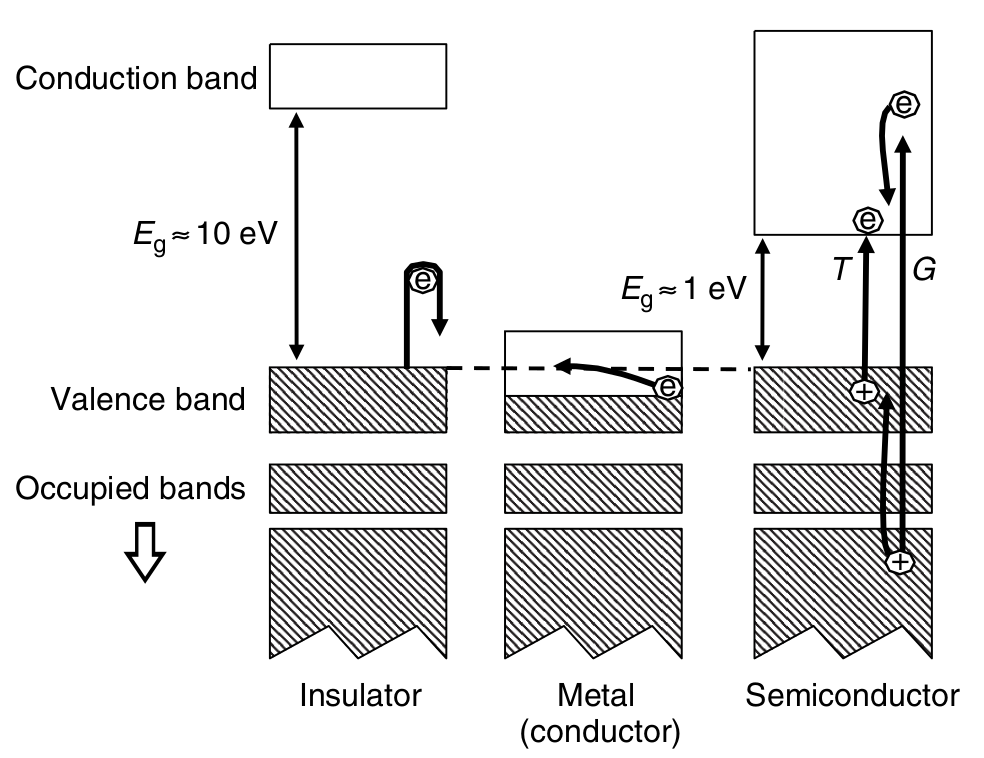
\includegraphics[width=0.4\textwidth]{./Bilder/ElectronBandsGilmore.png}
	\caption{Elektronen Bandstruktur aus \cite{book:gil}}\label{fig:eband}
\end{figure}
Das Leitungsband eines Halbleiters enthält meist auch Elektronen abhängig von
der Temperatur des Materials.
% Gleichung einfügen?
Um einen Halbleiter zu erhalten, der nach Möglichkeit nur von außen angeregte
Elektronen in seinem Leitungsband hat ist es sinnvoll diesen so weit wie
möglich herunter zu kühlen. Gamma Strahlen erzeugen in der Interaktion mit dem
Detektor schnelle Elektronen, die durch das anregen von Bandelektronen ihre
Energie abgeben. Dieses Elektronen können in einem Germanium Halbleiter
Elektronenlochpaare erzeugen, wenn diese die notwendige Energie von $\epsilon =
	\qty{2.96}{\eV}$ erreichen. Die Anzahl an Elektronenlochpaaren ist mit
\begin{align}
	N = E_e / \epsilon
\end{align}

proportional zu der Energie $E_e$ des Elektrons. Basierend auf der Stärke des
Halbleiterstroms lassen sich so Rückschlüsse auf die Energie des Elektrons
ziehen.

\subsection{Form des Detektors \cite[vgl][Kap. 2.4]{book:gil}}

Die Größe des Detektors spielt eine wichtige Rolle darin wie die Energie des
$\gamma$ Photons in ein Spektrum von Elektronenenergien übersetzt wird. Für die
moderat Energiereichen $\gamma$ Strahlen werden für diese Diskussion nur der
Compton Effekt und die photoelektrische Absorption beachtet. In einem
idealisierten kleinen Detektor streuen die $\gamma$ Photonen nur einmal und
geben dabei entweder ihre gesamte Energie an ein Photoelektron oder einen Teil
der Energie an ein Compton gestreutes Elektron. Compton gestreuten
Gammastrahlen hinterlassen nur einen teil ihrer Energie in dem Germanium
Detektor, und verlassen diesen direkt danach wieder. Das Ergebnis ist ein
Spektrum in der Form des Compton Wirkungsquerschnitts $d\sigma/dN$ aus
Gleichung \eqref{eq:compton_energie}. Bei einem realistischen Detektor können
die Compton gestreuten Photonen im Prinzip noch weitere male mit dem Detektor
interagieren und so eine Elektronenenergie zwischen dem Vollenergiepeak und dem
erwarteten wert im Compton Kontinuum erreichen.

\subsection{Dateninterpretation}

Die Quellen werden mit einem festen Abstand $d$ zum zylinderförmigen Detektor
mit Radius $r$ eingespannt. Sie strahlen gleichmäßig in alle Richtungen ab
können aber nur im Kegelförmigen Raumwinkel des Detektors gemessen werden. Ist
$2\theta$ der Öffnungswinkel des Kegels so ist \cite{wiki:raum}
\begin{align}
	\Omega = 4 \pi sin^2\left(\frac{\theta}{2}\right) \\
	\theta = \arctan \left(\frac{r}{d} \right)
\end{align}\label{eq:raumwinkel}

Die Anzahl $Z$ an Messungen in einem bestimmten Energiepeak hängt von dem
Raumwinkel $\Omega$, der Emissionswahrscheinlichkeit $W$, der Aktivität $A$ und
der Vollenergienachweiswahrscheinlichkeit $Q$ ab. Die
Vollenergienachweiswahrscheinlichkeit ist eine wichtige Kenngröße des
Detektors. Sie ist das Verhältnis von Photoelektrisch absorbierten
Gammastrahlen, die ihre Energie vollständig abgeben und z.B. Compton gestreuten
Elektronen, die die Energie nur teilweise abgeben.
\begin{align}
	Z = \frac{\Omega}{4\pi} A T W Q
	\label{eq:Q}
\end{align}

Die entstehenden Peaks haben die Form einer Gaußverteilung. Bei den Peaks lässt
sich die Zehntelwertsbreite und die Halbwertsbreite bestimmen. Wenn es sich bei
diesen um gaußverteilte Werte handelt haben sie eine Halbwertsbreite von
$2\sqrt{2\ln 2} \sigma$ und eine Zehntelwertsbreite von $2 \sqrt{2\ln
		10}\sigma$.

% \subsection{Wahrscheinlichste Photonenenergien}

% \begin{itemize}
% 	\item[\ce   {^{152}Eu}] - \qty{ 40.1186 } {\keV} \qty{37.7 (5)}{\%}
% 	\item[\ce   {^{152}Eu}] - \qty{121.7817 (3)} {\keV} \qty{28.41 (13)}{\%}
% 	\item[\ce   {^{152}Eu}] - \qty{344.2785 (12)} {\keV} \qty{26.59 (12)}{\%}
% 	\item[\ce   {^{137}Cs}] - \qty{661.6553 (30)} {\keV} \qty{85.01 (20)}{\%}
% 	\item[\ce   {^{133}Ba}] - \qty{30.9731}{\keV} \qty{62.4 (7)}{\%} x ray peak
% 	\item[\ce   {^{133}Ba}] - \qty{356.0129 (7)}{\keV} \qty{62.05 (19) 	}{\%} breiterer peak
% 	\item[\ce   {^{125}Sb}] - \qty{427.88}{\keV} \qty{29.6}{\%}
% \end{itemize}
% \cite{web:lara}

\newpage
\subsection{Fehlerrechnung}
Für die Fehlerrechnung werden alle \textbf{Mittelwerte} von $N$ Messungen
folgendermaßen berechnet:

\begin{equation}
	\overline{x} = \frac{1}{N} \cdot \sum_{i=1}^N x_i
	\label{eqn:Mittelwert}
\end{equation}

und alle \textbf{Standardabweichungen zum Mittelwert} mit:

\begin{equation}
	\increment\overline{x} = \sqrt{\frac{1}{N\cdot(N-1)}\cdot\sum_{i=1}^N (x_i-\overline{x})^2}
	\label{eqn:St_Mittelwert}
\end{equation}

Bei einigen Messungen bzw Messdaten ist der Fehler auch schon im Vorhinein
angegeben. Der Fehler für zusammenhängende Messwerte wird dann mit der
\textbf{Gaußschen Fehlerfortpflanzung} berechnet:

\begin{equation}
	\increment{f} = \sqrt{ \sum_{i = 1}^{N}  \biggl(\frac{\partial{f}}{\partial{x_i}}\biggr)^2\cdot(\increment{x_i})^2}
	\label{eqn:Gauss}
\end{equation}

Die Fehlerfortpflanzung wird mit Uncertainties in Python \cite{uncertainties}
ermittelt.

%---------------------------------------------------------------------------------------------------------------------------------------------------------------%

\section{Durchführung \cite[vgl.][]{man:v18}}

Der hier verwendete Detektor ist Zylinderförmig (l= \qty{39}{\mm}, Durchmesser
= \qty{45}{\mm}) und befindet sich in einer Aluminium Schutzhülle. Der Abstand
des Detektors zur Schutzhülle beträgt \qty{1.5}{\cm}. Die Schutzhülle sorgt
dafür, dass Gammastrahlen mit einer Energie niedriger als etwa
\qtyrange{40}{50}{\keV} nicht gemessen werden können. Für die
Vollenergienachweiswahrscheinlichkeit werden nur Energien größer
\qty{150}{\keV} betrachtet. Im Inneren des Detektors befindet sich eine
Koaxiale Bohrung deren innere Oberfläche mit Gold bedampft ist. Dieser Metall
Kontakt sorgt für die Ausprägung einer Verarmungszone in dem Detektor, die
diesen zu einem effektiven Halbleiter macht.

\begin{figure}
	\centering
	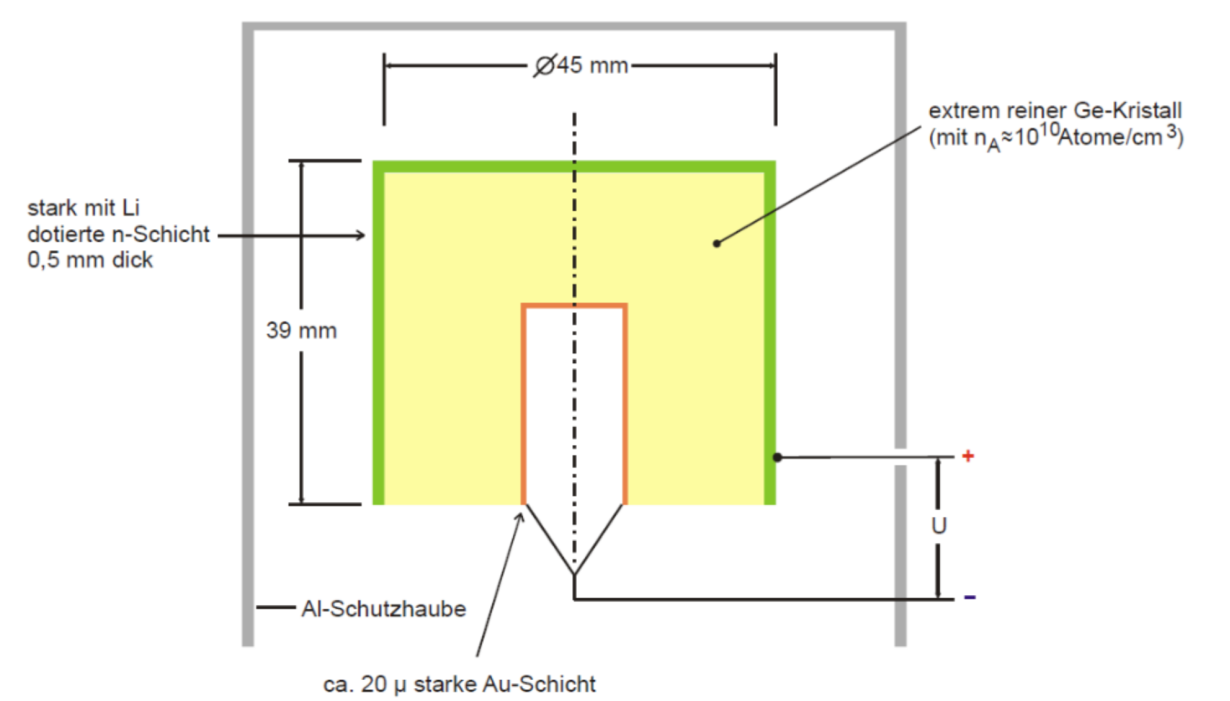
\includegraphics[width=0.4\textwidth]{./Bilder/querschnitt_detektor.png}
	\caption{Querschnitt des Germanium Detektors}\label{fig:cross}
\end{figure}

% TODO Abmessungen fertig machen

\subsection{Elektronik}
Der Detektor wird in diesem Versuchsaufbau durch vorgefertigte Bauteile
kontrolliert und ausgelesen. Ein Temperaturwächter kontrolliert die Kühlung des
Detektors und hält dessen Temperatur konstant auf \qty{77}{\kelvin}. 
Eine Hochspannungsquelle erhält die Verarmungszone des Halbleiters
aufrecht. Die Signale, die durch die Gammastrahlen in dem Detektor entstehen,
werden elektrisch verstärkt und mit einem Analog-Digital Wandler in Zählsignale
umgesetzt. Diese werden dem Computer übergeben, der ein Histogramm der
Ereignisse abhängig von den gemessenen Strömen erstellt.

\subsection{Messprogramm}
Die Energiespektren von 152Europium, der 137Cäsium und 133Barium werden
aufgenommen. hierzu werden die Proben in einem Abstand von \qty{70}{\mm} von
der Aluminium Abschirmung befestigt. Das Histogramm wird automatisiert jeweils
für etwa eine Stunde aufgenommen. Die genaue Messzeit wird in den Daten
automatisch hinterlegt. Schließlich wird die Unbekannte Quelle auf der
Schutzhülle positioniert. Deren Spektrum wird in gleicher Weise für etwa
\qty{45}{\min} aufgenommen.



